\documentclass[11pt,a4paper]{article}
\usepackage[margin=25mm]{geometry}
\usepackage{amsmath,amssymb}
\usepackage{graphicx}
\usepackage{booktabs}
\usepackage{array}
\usepackage{xcolor}
\usepackage{float}
\usepackage{caption}
\usepackage[hidelinks]{hyperref}
\usepackage[nameinlink]{cleveref}
\usepackage[autostyle, english = american]{csquotes}
\MakeOuterQuote{"}
\usepackage{microtype}
\emergencystretch=3em
\usepackage{setspace}
\onehalfspacing
\captionsetup{font=small,labelfont=bf}

\renewcommand{\thesection}{S\arabic{section}}
\renewcommand{\thefigure}{S\arabic{figure}}
\renewcommand{\thetable}{S\arabic{table}}
\crefname{section}{Section}{Sections}
\crefname{figure}{Fig.}{Figs.}
\crefname{table}{Table}{Tables}

\title{Supplementary material for\\
Local order parameters for ice polymorphs:\\a unified comparison and practical guide}
\author{Dibyendu Maity}
\date{}

\begin{document}
\maketitle

\section{Beyond ice: key and confined water}\label{sec:beyond}
The order parameters of the main text are often used to single out
functionally important water in biomolecular simulations. As a transfer test
outside the benchmark's design, we applied them unchanged, computed from water
oxygens and hydrogens only (host, guest, protein and ions are not neighbors),
to two sets of ligand-unbinding paths generated with PathGennie, using
geometric definitions of the waters of interest that no order parameter
enters. Scores are held-out balanced accuracies as in the main text: a
threshold is fitted on one half of the paths (OAMe--G2: path number modulo 2)
or on two replicas (T4L L99A: r1 and r2 against r3 and r4) and applied to the
other, and the worse direction is reported. Frames are saved path states, not
equally spaced in time. \Cref{tab:apps} summarizes the data.

\begin{table}[H]
\centering\small
\caption{Data of the supplementary applications.}
\label{tab:apps}
\begin{tabular}{>{\raggedright\arraybackslash}p{.17\linewidth}>{\raggedright\arraybackslash}p{.31\linewidth}>{\raggedright\arraybackslash}p{.17\linewidth}>{\raggedright\arraybackslash}p{.22\linewidth}}
\toprule
System & Paths & Model & Analyzed \\
\midrule
OAMe--G2 & 208 PathGennie escape paths of guest G2 & TIP3P, 300~K & up to 300 states per path \\
T4L L99A & 89 benzene-egress paths: 48 with a dry cavity (r1, r4), 41 with three cavity waters (r2, r3) & OPLS-AA, SPC/E, 300~K & 60 states per path \\
\bottomrule
\end{tabular}
\end{table}

\paragraph{Host--guest unbinding (OAMe--G2).} After rotating every frame onto
the host template used by the path-sampling bias, a cavity water is one
within 4.5~\AA{} of the host axis and below the portal, and a bridging water
one within 3.5~\AA{} of both a guest polar atom and a host oxygen. The cavity
is mostly dry. Averaged over the ten frames before the guest crosses the
portal it holds no more than 0.5 waters in 185 paths, at least two in 8 and
between in 6; 9 paths never cross. It stays nearly empty within the
recorded path even after the guest has left, so dry and wet refer to
occupancy during exit only. Against bulk water, cavity waters are separated
by Voronoi density (0.99), smooth CN (0.91), $\bar q_6$ (0.85) and CN (0.87),
and against water near the portal, which also touches the host, still by
Voronoi density (0.91), smooth CN (0.85) and $\bar q_6$ (0.81;
\cref{fig:beyond}a). Bridging waters are as distinct from bulk (1.00, 0.91
and, through $d_5$, 0.84). Cavity waters of dry and wet paths are not
distinguishable from each other (at most 0.64), and tetrahedral, entropy and
ring parameters are unstable: $\bar Q$ separates cavity from portal water at
0.94 on all paths pooled but only 0.67 when the threshold moves between path
halves. Which waters will enter the cavity within the next ten saved states
is decided by position: the distance to the portal alone gives a ROC area of
0.996, a held-out position model 0.997, and adding any or all order
parameters does not improve it (\cref{fig:beyond}b).

\paragraph{Buried water in a protein (T4 lysozyme L99A).} In the wet
ensemble three waters sit beside benzene in the hydrophobic cavity from the
start. Thresholds fitted on two replicas and tested on the other two separate
these three waters from protein-surface water through Voronoi density
(0.99), smooth CN (0.98), $\bar q_6$ and CN (0.96) and $\bar s$ (0.89), but not
through $\bar Q$ or $d_5$ (below 0.5). Other buried waters (at least 60
protein heavy atoms within 8~\AA) are harder (at most 0.80), because many
belong to small connected internal clusters. A rule frozen on buried versus
surface water flags 3.3--3.4 waters per frame within 8~\AA{} of the cavity in
the wet ensemble, against three present, recovering them in 99--100\% of
frames, and 1.0--1.2 in the dry ensemble, mostly other buried waters near the
pocket (\cref{fig:beyond}c). The three cavity waters remain buried and
isolated (smooth CN about 1.7) after benzene has left.

\paragraph{Interpretation and limits.} In both systems the parameters detect
confinement through the water coordination deficit, the missing water
neighbors that a hydrophobic cavity or a protein interior imposes, rather than
through a distinct local structure: isolated waters have large $\bar q_6$ and
$q_3$ only because a Steinhardt invariant of one or two bonds is large.
Detection is reliable for isolated confined waters and weak for water in
connected internal clusters, and local structure does not anticipate which
waters enter a cavity. For confined water we would therefore use Voronoi
density, smooth CN or CN from water neighbors only, and avoid tetrahedral,
entropy and ring parameters and any reading of a high $\bar q_l$ of isolated
waters as order. These are two systems, two water models at 300~K and sampled
path frames rather than equilibrium trajectories; the results show what
water-only parameters can and cannot report, not a general water classifier.

\begin{figure}[H]
\centering
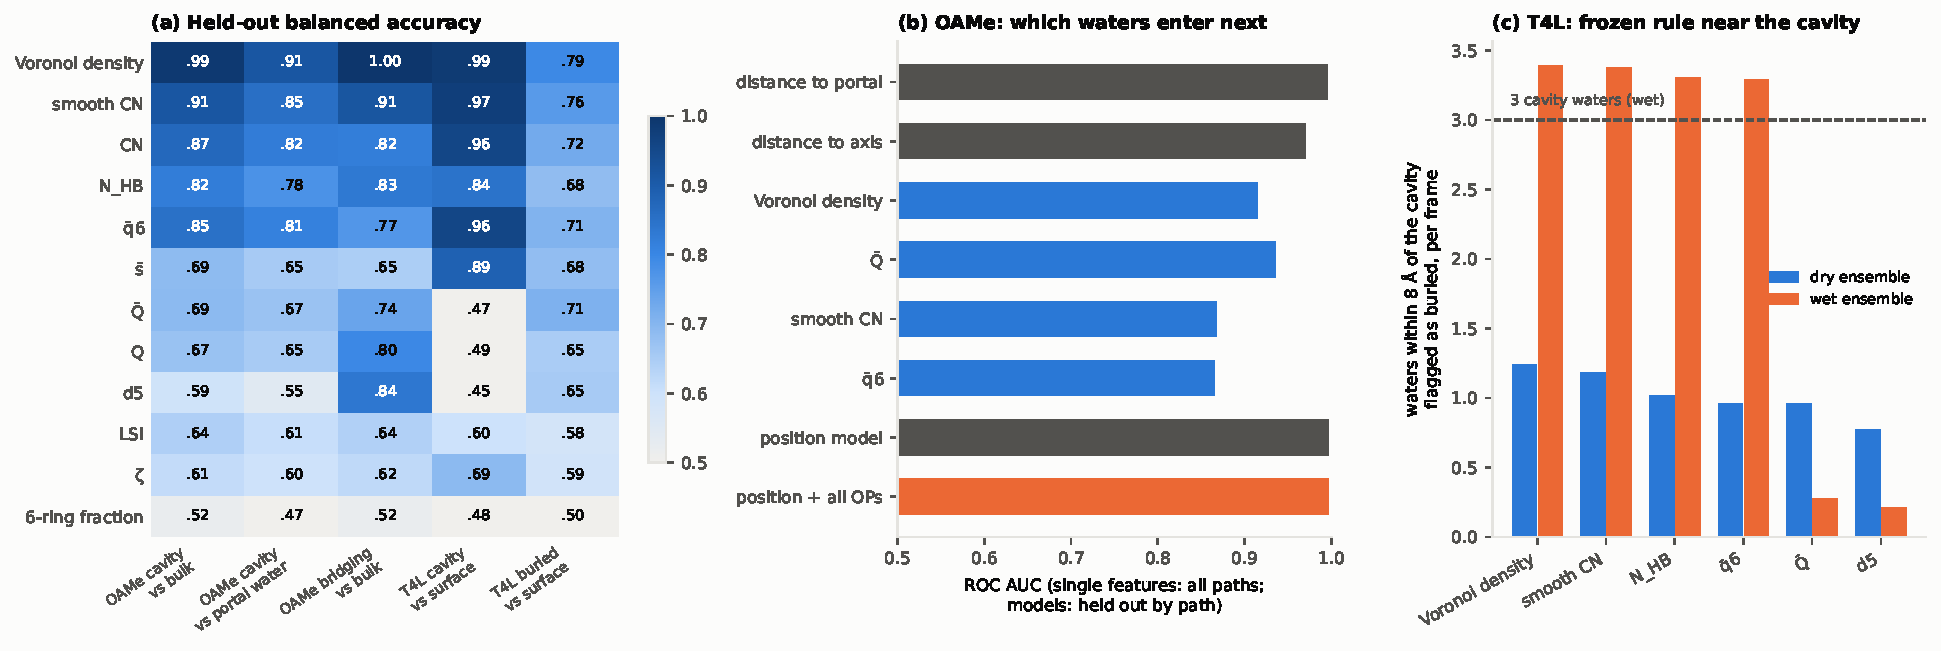
\includegraphics[width=\linewidth]{../benchmarks/results/figures/F11_applications.pdf}
\caption{Key and confined water beyond ice. (a) Held-out balanced accuracy
(threshold fitted on half of the paths or replicas, applied to the other,
worse direction) of water-only parameters for OAMe--G2 cavity waters against
bulk and against water within 10~\AA{} of the portal, bridging waters
against bulk, and T4L L99A cavity and buried waters against protein-surface
water. (b) OAMe--G2: ROC area for identifying the waters near the portal that
enter the cavity within the next ten saved states; single features evaluated
on all paths, logistic models held out by path. (c) T4L L99A: waters within
8~\AA{} of the cavity flagged as buried per frame by rules frozen on buried
versus surface water, in the dry and wet ensembles; dashed, the three cavity
waters of the wet ensemble.}
\label{fig:beyond}
\end{figure}

\paragraph{Data.} The unbinding trajectories belong to separate
path-sampling campaigns and are not archived. The archive
(\texttt{coordinates/applications/}) holds, per water and analyzed frame, every
order parameter, the geometric region label, the quantities that define it
(position relative to the host axis and portal, burial, distances to the
ligand) and the split columns (\texttt{path}, \texttt{replica}), as
\texttt{oame\_features.npz} and \texttt{t4l\_features.npz}.
\texttt{host\_guest.py analyze} and \texttt{confined\_water.py analyze}
reproduce every number and \cref{fig:beyond} from these files alone; we
checked that the regenerated tables are byte-identical to the published ones.

\end{document}
